\resizebox{1\textwidth}{!}{%
	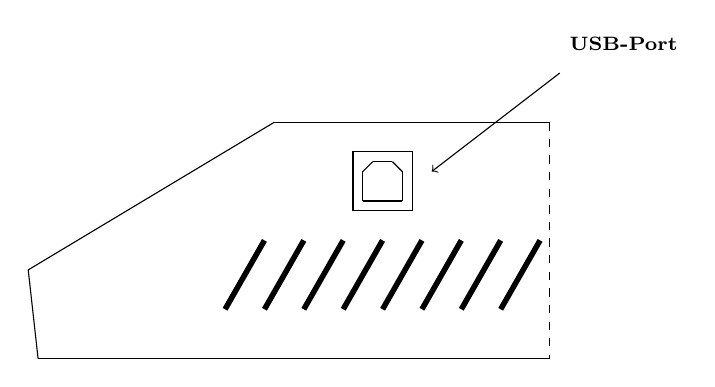
\begin{tikzpicture}
		\tikzstyle{every node}=[font=\fontsize{7pt}{18.5pt}\selectfont]
		
		\draw (2.625,13.125) -- (9.125,13.125);
		\draw (2.625,13.125) -- (2.5,14.25);
		\draw (2.5,14.25) -- (5.625,16.125);
		\draw (5.625,16.125) -- (9.125,16.125);
		\draw [dashed] (9.125,16.125) -- (9.125,13.125);
		
		\draw (6.625,15.75) rectangle (7.375,15);
		
		\draw [line width=2pt] (5,13.75) -- (5.5,14.625);
		\draw [line width=2pt] (5.5,13.75) -- (6,14.625);
		\draw [line width=2pt] (6,13.75) -- (6.5,14.625);
		\draw [line width=2pt] (6.5,13.75) -- (7,14.625);
		\draw [line width=2pt] (7,13.75) -- (7.5,14.625);
		\draw [line width=2pt] (7.5,13.75) -- (8,14.625);
		\draw [line width=2pt] (8,13.75) -- (8.5,14.625);
		\draw [line width=2pt] (8.5,13.75) -- (9,14.625);
		
		%\draw [->] (2.5,16.875) -- (4,15.375);
		%\node at (2.125,17.25) {\textbf{Bedienfeld}};
		
		\draw (6.875,15.625) -- (7.125,15.625);
		\draw (7.125,15.625) -- (7.25,15.5);
		\draw (6.875,15.625) -- (6.75,15.5);
		\draw (6.75,15.5) -- (6.75,15.125);
		\draw (7.25,15.5) -- (7.25,15.125);
		\draw (6.75,15.125) -- (7.25,15.125);
		
		\draw [->] (9.25,16.75) -- (7.625,15.5);
		\node [anchor=west] at (9.25,17.125) {\textbf{USB-Port}};
		
	\end{tikzpicture}
}%